\documentclass{beamer}

\usepackage[utf8]{inputenc}
\usepackage{fancybox,fancyvrb}
\usepackage{environ}
\usepackage{tikz}

\beamertemplatenavigationsymbolsempty
\setbeamertemplate{footline}[frame number]
\usetheme{Pittsburgh}

\newcommand\enumnum[1]{{\renewcommand{\insertenumlabel}{#1}%
      \usebeamertemplate{enumerate item} \,}}

\newcommand{\grad}{\nabla}
\newcommand{\ih}{\boldsymbol{\hat{\textbf{\i}}}}
\newcommand{\jh}{\boldsymbol{\hat{\textbf{\j}}}}
\newcommand{\vF}{\boldsymbol{\vec{\textbf{F}}}}
\newcommand{\Matlab}{\textsc{Matlab}}


\title{4.4 Nonhomogeneous equations: \\ method of undetermined coefficients}

\subtitle{a lesson for MATH F302 Differential Equations}

\author{Ed Bueler, Dept.~of Mathematics and Statistics, UAF}

\date{\tiny \today}


\begin{document}
\setbeamertemplate{itemize item}{$\bullet$}
\setbeamertemplate{itemize subitem}{$\circ$}


\begin{frame}
\titlepage

\centerline{\tiny for textbook: \, D. Zill, \emph{A First Course in Differential Equations with Modeling Applications}, 11th ed.}
%\color{green!40!blue}
\end{frame}


\begin{frame}{general solutions to nonhomogeneous DEs}

\begin{itemize}
\item an $n$th-order, linear, and nonhomogeneous DE:
\begin{equation*}
    a_n(x) y^{(n)} + a_{n-1}(x) y^{(n-1)} + \dots + a_1(x) y' + a_0(x) y \stackrel{\ast}{=} g(x)
\end{equation*}
\item \alert{main claim:} the general solution is a sum of the general solution of the associated \emph{homogeneous} equation,
\begin{equation*}
    a_n(x) y^{(n)} + a_{n-1}(x) y^{(n-1)} + \dots + a_1(x) y' + a_0(x) y = 0
\end{equation*}
plus one \emph{particular solution} $y_p(x)$ of $\ast$
    \begin{itemize}
    \item the general solution of the homogeneous equation is called the \emph{complementary function} $y_c(x)$
    \end{itemize}

\bigskip
\item $\alert{y(x) = y_c(x) + y_p(x)}$
\end{itemize}
\end{frame}


\begin{frame}{example 1}

\begin{itemize}
\item \emph{example 1}: find the general solution:
    $$y'' + 4 y = e^{-x}$$
\end{itemize}

\vspace{60mm}
\end{frame}


\begin{frame}{example 1, cont.}

\begin{itemize}
\item verify that $y(x) = c_1 \cos 2x + c_2 \sin 2x + \frac{1}{4} e^{-x}$ solves
    $$y'' + 4 y = e^{-x}$$

\vspace{60mm}
\end{itemize}
\end{frame}


\begin{frame}{example 1, cont.$^2$}

\begin{itemize}
\item solve the initial value problem:
    $$y'' + 4 y = e^{-x}, \qquad y(0)=-1, \quad y'(0)=\frac{3}{4}$$

\vspace{60mm}
\end{itemize}
\end{frame}


\begin{frame}{example 2}

\begin{itemize}
\item the idea of ``undetermined coefficients'' is to

\centerline{\alert{try a general form of the nonhomogeneity $g(x)$}}
\item \emph{example 2 ($\approx$ \#5 in 4.4)}: find the general solution:
    $$y'' + 4 y' + 4y = x^2 - 2 x \hspace{50mm}$$
\end{itemize}

\vspace{50mm}
\end{frame}


\begin{frame}{example 3}

\begin{itemize}
\item \emph{example 3 ($=$ \#8 in 4.4)}: find the general solution:
    $$4 y'' - 4 y' - 3 y = \cos 2x \hspace{50mm}$$
\end{itemize}

\vspace{60mm}
\end{frame}


\begin{frame}{trial forms for the particular solution}

\begin{itemize}
\item if we are going to guess a form we need some guidance
\item in words:

\begin{quotation}
\noindent For $y_p$ try a linear combination of all linearly-independent functions generated by repeated differentiation of $g(x)$.
\end{quotation}

\vspace{-3mm}
\item as a table:
\end{itemize}

\hfill 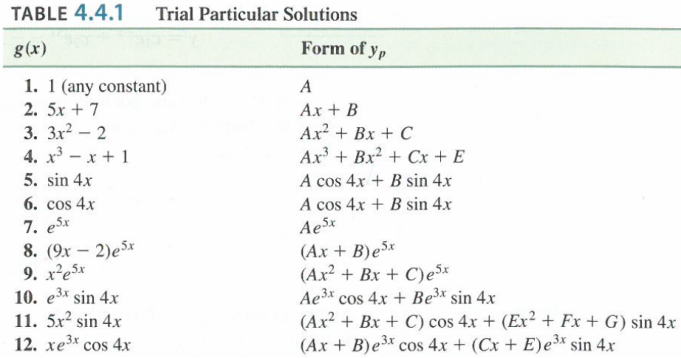
\includegraphics[width=0.8\textwidth]{figs/yptable}
\end{frame}


\begin{frame}{X}

\begin{itemize}
\item X
\end{itemize}
\end{frame}


\begin{frame}{X}

\begin{itemize}
\item X
\end{itemize}
\end{frame}


\begin{frame}{X}

\begin{itemize}
\item X
\end{itemize}
\end{frame}


\begin{frame}{X}

\begin{itemize}
\item X
\end{itemize}
\end{frame}


\begin{frame}{X}

\begin{itemize}
\item X
\end{itemize}
\end{frame}


\begin{frame}{what we are skipping now}

we are \alert{skipping} the following sections:
\begin{itemize}
\item \S 4.5 \emph{Undetermined Coefficients---Annihilator Approach}

a more abstract view of undetermined coefficients, but no more powerful
\item \S 4.6 \emph{Variation of parameters}

a general approach to nonhomogeneous linear equations \underline{but} one may not be able to compute the integrals you get
    \begin{itemize}
    \item it is somewhat like reduction of order
    \end{itemize}
\item \S 4.7 \emph{Cauchy-Euler equations}

another class of differential equations which can be solved via an auxiliary equation
\item \S 4.8 \emph{Green's Functions}

mostly relevant to boundary value problems (not in Math 302)
\item \S 4.9 \emph{Solving Systems of Linear DEs by Elimination}

a way of solving systems; systmes are important and done generally in chapter 8
\end{itemize}
\end{frame}


\begin{frame}{expectations}

\begin{itemize}
\item just watching this video is \emph{not} enough!
     \begin{itemize}
     \item see ``found online'' videos at

     \centerline{\href{https://bueler.github.io/math302/week7.html}{\tt \color{cyan} bueler.github.io/math302/week7.html}}
     \item \emph{read} section 4.4 in the textbook
     \item \emph{do} the WebAssign exercises for section 4.4
     \end{itemize}
\end{itemize}
\end{frame}

\end{document}

